\documentclass[aspectratio=169,11pt]{beamer}
\usepackage[T1]{fontenc}
\usepackage{helvet}
\renewcommand{\familydefault}{\sfdefault}
\usepackage{tikz}
\usetikzlibrary{positioning,arrows.meta}
\definecolor{cmured}{HTML}{C41230}
\definecolor{ink}{HTML}{222222}
\definecolor{soft}{HTML}{F4F4F4}
\definecolor{mid}{HTML}{6B6B6B}
\setbeamercolor{frametitle}{fg=cmured,bg=white}
\setbeamercolor{normal text}{fg=ink}
\setbeamercolor{itemize item}{fg=cmured}
\setbeamerfont{frametitle}{size=\Large,series=\bfseries}
\setbeamertemplate{navigation symbols}{}
\setbeamertemplate{itemize item}{\small$\blacksquare$}
\setbeamertemplate{footline}{\hspace{1em}\color{mid}\scriptsize Group 19 \textbullet{} CMU Heinz College \textbullet{} Interactivity Foundation, October 8, 2026\hfill\insertframenumber/5\hspace{1em}\vspace{6pt}}
\hyphenpenalty=10000
\exhyphenpenalty=10000
\newcommand{\card}[3]{\begin{tikzpicture}\node[fill=soft,rounded corners=4pt,text width=#1,inner sep=7pt,align=left]{{\color{cmured}\bfseries\small #2}\\[3pt]\footnotesize #3};\end{tikzpicture}}

\begin{document}

% 1
\begin{frame}{Toolkit Migration: Our Understanding}
{\small\color{mid} Moving the Collaborative Discussion Toolkit from Wix to the IF Website}\par
\vspace{10pt}
\begin{columns}[T]
\begin{column}{0.5\textwidth}
\textbf{\small What we heard on October 1}
\begin{itemize}\small
  \item 46 activities in five modules, each with a PDF, on a separate Wix site
  \item Our reading of your reasons: lower platform costs, and your work fully accessible on your main website
  \item You chose the IF Website as the new home
  \item Activities are being revised, so future updates must be easy to post
  \item You want an agentic workflow, using many agents to assist with this work
\end{itemize}
\end{column}
\begin{column}{0.46\textwidth}
\card{0.92\textwidth}{By December 3}{All 46 activities on the IF Website in one consistent layout, published once IF approves them, with their PDFs and old Toolkit links sending visitors to the new pages.\\[4pt]A simple way for staff to turn a new or revised activity into a page ready for review (target: 15 minutes or less, to confirm).\\[4pt]Training, guides, and everything handed over to IF.}
\end{column}
\end{columns}
\end{frame}

% 2
\begin{frame}{Our Team and Who Does What}
\vspace{-10pt}
\centering
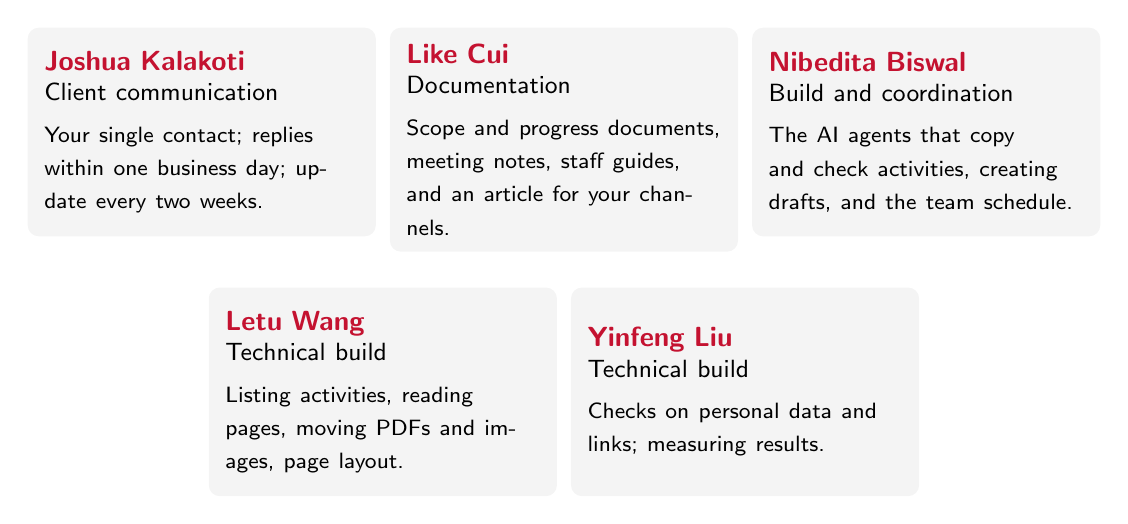
\begin{tikzpicture}[box/.style={fill=soft,rounded corners=4pt,text width=4.0cm,minimum height=2.65cm,inner sep=6pt,align=left,anchor=north}]
\node[box] (j) at (-4.6,0) {{\color{cmured}\bfseries Joshua Kalakoti}\\\small Client communication\\[3pt]\footnotesize Your single contact; replies within one business day; update every two weeks.};
\node[box] (l) at (0,0) {{\color{cmured}\bfseries Like Cui}\\\small Documentation\\[3pt]\footnotesize Scope and progress documents, meeting notes, staff guides, and an article for your channels.};
\node[box] (n) at (4.6,0) {{\color{cmured}\bfseries Nibedita Biswal}\\\small Build and coordination\\[3pt]\footnotesize The AI agents that copy and check activities, creating drafts, and the team schedule.};
\node[box] (le) at (-2.3,-3.3) {{\color{cmured}\bfseries Letu Wang}\\\small Technical build\\[3pt]\footnotesize Listing activities, reading pages, moving PDFs and images, page layout.};
\node[box] (y) at (2.3,-3.3) {{\color{cmured}\bfseries Yinfeng Liu}\\\small Technical build\\[3pt]\footnotesize Checks on personal data and links; measuring results.};
\end{tikzpicture}
\par\vspace{6pt}
{\scriptsize All five attend every client meeting. Everything we build is reviewed by a second team member.}
\end{frame}

% 3
\begin{frame}{Project Plan: How It Works}
\vspace{-2pt}
\centering
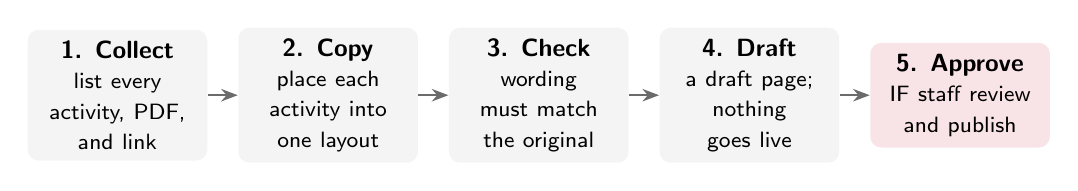
\begin{tikzpicture}[
  st/.style={fill=soft,rounded corners=4pt,text width=2.0cm,minimum height=1.3cm,align=center,inner sep=4pt,font=\small},
  hum/.style={st,fill=cmured!12},
  ar/.style={-{Stealth[length=6pt]},thick,color=mid}]
\node[st] (a) {\textbf{1. Collect}\\\footnotesize list every activity, PDF, and link};
\node[st,right=0.38cm of a] (b) {\textbf{2. Copy}\\\footnotesize place each activity into one layout};
\node[st,right=0.38cm of b] (c) {\textbf{3. Check}\\\footnotesize wording must match the original};
\node[st,right=0.38cm of c] (d) {\textbf{4. Draft}\\\footnotesize a draft page; nothing goes live};
\node[hum,right=0.38cm of d] (e) {\textbf{5. Approve}\\\footnotesize IF staff review and publish};
\draw[ar] (a)--(b); \draw[ar] (b)--(c); \draw[ar] (c)--(d); \draw[ar] (d)--(e);
\end{tikzpicture}
\par\vspace{0pt}
{\scriptsize\color{mid} The agents: fixed code copies each activity from its Wix record; a coordinating agent runs the steps; a reading agent handles new documents; a reviewer agent explains flags to your staff. Checks and drafts follow fixed rules, so they behave the same every time.}
\par\vspace{2pt}
\begin{columns}[T]
\begin{column}{0.47\textwidth}
\card{0.9\textwidth}{After handover: adding an activity}{Give the activity document to the AI with our saved instructions, paste the checked result into the Website's activity form, review, and publish. A form and checklist work without AI too.}
\end{column}
\begin{column}{0.47\textwidth}
\card{0.9\textwidth}{Safety built in}{The AI never publishes or rewrites your activities. Claude is used only with your permission.}
\end{column}
\end{columns}
\end{frame}

% 4
\begin{frame}{Roadmap to December 3}
\vspace{6pt}
\centering
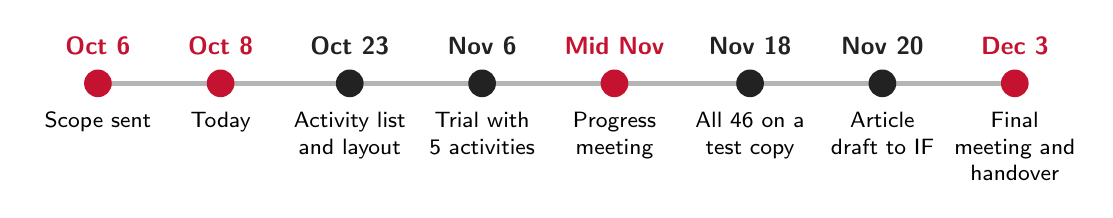
\begin{tikzpicture}[x=0.82cm,y=1cm]
\draw[line width=2pt,color=mid!50] (0,0) -- (14.2,0);
\foreach \x/\d/\t/\c in {
  0/{Oct 6}/{Scope sent}/cmured,
  1.9/{Oct 8}/{Today}/cmured,
  3.9/{Oct 23}/{Activity list and layout}/ink,
  5.95/{Nov 6}/{Trial with 5 activities}/ink,
  8.0/{Mid Nov}/{Progress meeting}/cmured,
  10.1/{Nov 18}/{All 46 on a test copy}/ink,
  12.15/{Nov 20}/{Article draft to IF}/ink,
  14.2/{Dec 3}/{Final meeting and handover}/cmured}{
  \fill[color=\c] (\x,0) circle (5pt);
  \node[above=7pt,font=\small\bfseries,color=\c] at (\x,0) {\d};
  \node[below=7pt,font=\footnotesize,align=center,text width=1.55cm] at (\x,0) {\t};
}
\end{tikzpicture}
\par\vspace{4pt}
{\footnotesize\color{mid} Red: meetings and agreed deadlines. Dark: our proposed milestones.}
\par\vspace{2pt}
\card{0.86\textwidth}{What this asks of IF (estimates to confirm today)}{About 15 staff hours in total, mostly reviewing drafts in batches in November. A test copy of the website (or an editor account) so nothing touches your live site until you approve. An email update from Joshua every two weeks between meetings.}
\end{frame}

% 5
\begin{frame}{Success Measures and Decisions}
\vspace{-6pt}
\begin{columns}[T]
\begin{column}{0.44\textwidth}
\textbf{Proposed success measures}
\begin{itemize}\footnotesize
  \item All 46 activities and PDFs moved
  \item Wording unchanged; any difference shown to IF before approval
  \item No broken links; old Toolkit links lead to the new pages
  \item New activity ready for review in 15 minutes or less (target to confirm)
  \item Nothing goes live without IF approval
\end{itemize}
\end{column}
\begin{column}{0.52\textwidth}
\textbf{Needed today}
\begin{itemize}\footnotesize
  \item Access: a test copy of the website or an editor account
  \item Permission to process Toolkit content with Claude
  \item Scope: activities only, or also ratings, coach resources, certificate templates
\end{itemize}
\vspace{4pt}
\vspace{-2pt}\textbf{By October 16}
\begin{itemize}\footnotesize
  \item Date after which revisions wait for the new site
  \item Plans for the old web address
  \item Your owner after December; NDA if needed
\end{itemize}
\end{column}
\end{columns}
\vspace{2pt}
\centering\card{0.9\textwidth}{Next step}{We update the scope with today's answers and send Version 2 by Monday, October 12, for your approval.}
\end{frame}

\end{document}
